\documentclass[a4paper,11pt]{article}

\usepackage[slovene]{babel}
\usepackage[T1]{fontenc}
\usepackage[utf8]{inputenc}
\usepackage{lmodern}

\usepackage{textcase}
\usepackage{amsmath}
\usepackage{amsfonts}
% \usepackage{amsthm}
\usepackage{fancyhdr}
\usepackage[italicdiff]{physics}
\usepackage{url}
\usepackage{graphicx}
\usepackage{bm}
\usepackage{physics}
\usepackage{icomma}
\usepackage{hyperref}
% \usepackage[showframe]{geometry}

\graphicspath{ {./images/}}

\pagestyle{fancy}
\fancyhf{}
\rhead{\thepage}
\lhead{\textsc{\textsc{Seminarska naloga iz statistike}}}

% \setlength{\parskip}{1em}

\newcommand{\ols}[1]{\mskip.5\thinmuskip\overline{\mskip-.5\thinmuskip {#1} \mskip-.5\thinmuskip}\mskip.5\thinmuskip} % overline short
\newcommand{\olsi}[1]{\,\overline{\!{#1}}} % overline short italic

\newcommand{\sumin}{\sum_{i = 1}^n}
\newcommand{\sumiN}{\sum_{i = 1}^N}

\newcommand{\inv}{^{-1}}
\newcommand{\prob}{\mathsf{P}}

\newcommand{\R}{\mathbb{R}}
\newcommand{\Z}{\mathbb{Z}}

\AtBeginDocument{
    \renewcommand{\var}[1]{\operatorname{var}(#1)}
}
    
\DeclareMathOperator{\se}{se}
\DeclareMathOperator{\bin}{Bin}

%%%%%%%%%%%%%%%%%%%%%%%%%%%%%%%%%%%%%%%%%%%%%%%%%%%%%%%%%%%%%%%%

\begin{document}
    
\author{\Large{\textbf{Izak Jenko}}}
\title{SEMINARSKA NALOGA IZ STATISTIKE}
\date{22. avgust 2021}

\maketitle
\thispagestyle{empty}

\par
Seminarska naloga iz statistike pri predmetu statistika na Fakulteti za matematiko in fiziko v Ljubljani v študijskem letu 2020/21. Celoten repozitorij seminarske naloge, ki vključuje skripte in izračune, najdemo na spletnem naslovu:
\begin{center}
    \url{https://github.com/kazi99/STAT-seminarska} 
\end{center}

%-------------------------------------------------------------%
\section*{1. naloga}
%-------------------------------------------------------------%

Naj $x_i$ označuje dohodek $i$-te družine za $1 \leq i \leq N := 43 886$. Vzamemo enostavni slučajni vzorec $X_i := x_{K_i}$, kjer je slučajni vektor $(K_1, \ldots, K_n)$ enakomerno porazdeljen po množici $n$-teric s samimi različnimi komponentami, ki prihajajo iz množice $\{ 1, \dots, N\}$. Vzorec bo velikosti $n = 400$ in bo \emph{proporcionalno alociran}, da bomo lahko na koncu primerjali točki a) in b).
\\

\noindent
\textbf{a)} Populacijsko povprečje $\mu = \frac1N \sum_{i=1}^N x_i$ točkovno ocenimo z vzorčnim povprečjem
\[
    \olsi{X} = \frac1n \sum_{i = 1}^n X_i,  
\]
ki na našem vzorcu znaša $43410,49$. Označimo s $\sigma^2 = \frac{1}{N}\sum_{i = 1}^N (x_i - \mu)^2$ populacijsko varianco. Varianca cenilke $\olsi{X}$ bo 
\[
    \var{\olsi{X}} = \frac{\sigma^2}{n}\left(1 - \frac{n-1}{N-1}\right),
\]
kjer faktor $1 - \frac{n-1}{N-1}$ nastopi zaradi koreliranosti posameznih enot enostavnega slučajnega vzorca. Standardna napaka cenilke $\olsi{X}$, bo torej $\se = \frac{\sigma}{\sqrt{n}} \sqrt{1 - \frac{n-1}{N-1}}$. Popoulacijske variance $\sigma^2$ običajno ne poznamo, je pa 
\[
    s^2 = \frac{1}{n-1}\sumin(X_i - \olsi{X})^2, 
\]
njena nepristranska cenilka, torej standardno napako ($\se$) lahko ocenimo z
\[
    \hat{\se} = \frac{s}{\sqrt{n}}\sqrt{1 - \frac{n}{N}}.
\]
Izračunana na našem vzorcu je ocena standardne napake enaka $1758,62$.

Sedaj imamo zbrane vse podatke, da postavimo $95\%$ interval zaupanja. Stopnja tveganja bo $\alpha = 0,05$ in to je verjetnost, da populacijska statistika (na primer povprečni dohodek) ni vsebovana v našem intervalu zaupanja, ki je slučajna množica. Opravka imamo z veliko ($400$ je velikost vzorca) enako porazdeljenimi (porazdelitev je empirična) slučajnimi spremenljivkami, zato lahko zaradi centralnega limitnega izreka predpostavljamo, da je vzorčno povprečje $\olsi{X}$ porazdeljeno približno normalno. Opomnimo še, da te slučajne spremenljivke niso nujno neodvisne, je pa njihova koreliranost razmeroma majhna pri tako veliki populaciji kot je naša, zato je uporaba izreka nekoliko bolj utemeljena. 

Držimo se standardnih oznak in označimo s $\Phi$ kumulativno porazdelitveno funkcijo standardne normalne porazdelitve
\[
    \Phi(x) = \frac{1}{\sqrt{2 \pi}} \int_{-\infty}^{x} e^{-z^2/2}\,dz.
\]
Če bi poznali populacijsko varianco $\sigma^2$ in s tem standardno napako, bi dobili inteval zaupanja   
\begin{equation}
    \label{normalni IZ}    
    \left(\olsi{X} - \se \Phi\inv\left(1 - \frac{\alpha}{2}\right), 
    \olsi{X} + \se \Phi\inv\left(1 - \frac{\alpha}{2}\right)\right).
\end{equation}
Kar pri našem vzorcu pride $\left( 35581,54; 41832,12 \right)$ in je dolžine $6250,58$.

Glede na to, da imamo tudi oceno standardne napake in recimo prave vrednosti standardne napake ne bi poznali, lahko postavimo tudi aproksimativni interval zaupanja oblike
\begin{equation}
    \label{aproksimativni IZ}
    \left(\olsi{X} - \hat{\se} \Phi\inv\left(1 - \frac{\alpha}{2}\right), 
    \olsi{X} + \hat{\se} \Phi\inv\left(1 - \frac{\alpha}{2}\right)\right).
\end{equation}
ki je asimptotično eksakten. Na našem vzorcu znaša $\left( 35937,86; 41475,80\right)$ in je dolžine $5537,94$. 
V tem primeru, ko poznamo samo oceno standardne napake, si lahko pomagamo tudi s Studentovo $t$-porazdelitvijo in tako dobimo Studentov interval zaupanja
\begin{equation}
    \label{studentov IZ}
    \left(\olsi{X} - \hat{\se} F_{\text{Student}(n-1)}\inv\left(1 - \frac{\alpha}{2}\right), 
    \olsi{X} + \hat{\se} F_{\text{Student}(n-1)}\inv\left(1 - \frac{\alpha}{2}\right)\right),
\end{equation}
kjer $F_{\text{Student}(n-1)}$ označuje kumulativno porazdelitveno funkcijo Studentove $t$-porazdelitve z $n-1$ prostostnimi stopnjami. Na našem vzorcu pride interval zaupanja $\left(35929,43; 41484,23\right)$, ki je dolžine $5554,79$.
\\

\noindent
\textbf{b)} V tej točki si bomo pogledali kako dobro lahko ocenimo statistike od prej, če si pomagamo s stratificiranjem prebivalstva po četrtih. Naš vzorec velkosti $400$ je stratifician s proporcionalno alokacijo, kar pomeni, da vzamemo $n_1 = 92$ enot iz severne četrti, $n_2 = 95$ iz vzhodne, $n_3 = 123$ iz južne in $n_4 = 90$ iz zahodne četrti kot kaže tabela.
\begin{center}
\begin{tabular}{|c || c c c c ||}
    \hline
    & Sever & Vzhod & Jug & Zahod \\
    \hline
    $n_j$ & $92$ & $95$ & $123$ & $90$ \\
    \hline 
\end{tabular}
\end{center}
Do teh števil pridemo, tako da nekoliko prilagodimo količine $n_j \approx n \cdot w_j$ (tu je $w_j$ delež populacije, ki živi v $j$-ti četri). Polovico od količin $n_j$ zaokrožimo navzgor do najbližjega celega števila, preostale pa navzdol do celega števila.

Najprej stratumsko ocenimo populacijsko povprečje $\mu$ kot
\[
    \olsi{X}_s = \sum_{j = 1}^4 w_j \olsi{X}_j, \quad \text{ kjer je } \quad \olsi{X}_j = \frac{1}{n_j}\sum_{i = 1}^{n_j} X_{ij}
\]
Stratificirana standardna napaka se izraža kot
\[
    \se^2_s = \sum_{j = 1}^4 \frac{w_j^2 \sigma_j^2}{n_j}\left(1 - \frac{n_j - 1}{N_j - 1}\right), 
\]
kjer je stratificirana populacijska varianca $\sigma_j^2 = \sum_{i = 1}^{n_j} \frac{(X_{ij} - \mu_j)^2}{N_j}$. 

Ocena standardne napake bo tedaj 
\[
    \hat{se}^2_s = \sum_{j = 1}^4 \frac{w_j^2 \hat{\sigma}_j^2}{n_j}\left(1 - \frac{n_j - 1}{N_j - 1}\right),
\] 
kjer je $\hat{\sigma}^2_j = \sum_{i = 1}^{n_j} \frac{(X_{ij} - \olsi{X}_j)^2}{n_j - 1}$ nepristranska cenilka populacijske variance v $j$-tem stratumu $\sigma_j^2$.

Sedaj lahko podobno kot prej postavimo $95\%$ intervale zaupanja. Najprej če predpostavjlamo, da poznamo populacijsko varianco, dobimo
\[
    \left(\olsi{X}_s - \se_s \cdot \Phi\inv\left(1 - \frac{\alpha}{2}\right), 
    \olsi{X} + \se_s \cdot \Phi\inv\left(1 - \frac{\alpha}{2}\right)\right).
\] 
Na našem vzorcu je to $\left(35594,36; 41818,41 \right)$, ki je dolžine $6224,06$, kar pomeni, da je krajši kot interval \eqref{normalni IZ} in s tem tudi boljši za ocenejevanje povprečnega dohodka. 

Naslednji je aproksimativni interval zaupanja, kjer uporabimo oceno za standardno napako $\hat{\se}_s$. Interval bo tedaj 
\[
    \left(\olsi{X}_s - \hat{\se}_s \cdot \Phi\inv\left(1 - \frac{\alpha}{2}\right), 
    \olsi{X} + \hat{\se}_s \cdot \Phi\inv\left(1 - \frac{\alpha}{2}\right)\right), 
\]
ki bo pri naših podatkih $\left(35931,97; 41480,80\right)$ dolžine $5548,84$, kar je pravtako krajše kot interval \eqref{aproksimativni IZ} in tako boljše, kot če ne bi stratificirali.

Nazadnje lahko postavimo še Studentov interval zaupanja za ocenejevanje povprečja, pred tem pa moramo izračunati prostostne stopnje
\[
    \hat{\nu} = \frac{\hat{\se}^2_s}{\sum_{j = 1}^4 \frac{w_j^4 \hat{\sigma}^2_j}{n_j^2 (n_j - 1)}}.  
\]
Interval zaupanja bo tako oblike
\[
    \left(\olsi{X} - \hat{\se} \cdot F_{\text{Student}(\hat{\nu})}\inv\left(1 - \frac{\alpha}{2}\right), 
    \olsi{X} + \hat{\se} \cdot F_{\text{Student}(\hat{\nu})}\inv\left(1 - \frac{\alpha}{2}\right)\right),  
\]
na naših podatkih bo to interval $\left(35931,97; 41480,80\right)$ dolžine $5548,84$, ki je spet boljši kot \eqref{studentov IZ}, ko nismo stratificirali.

Intervale zaupanja prikažemo tudi grafično.
\begin{figure}[h]
    \centering
    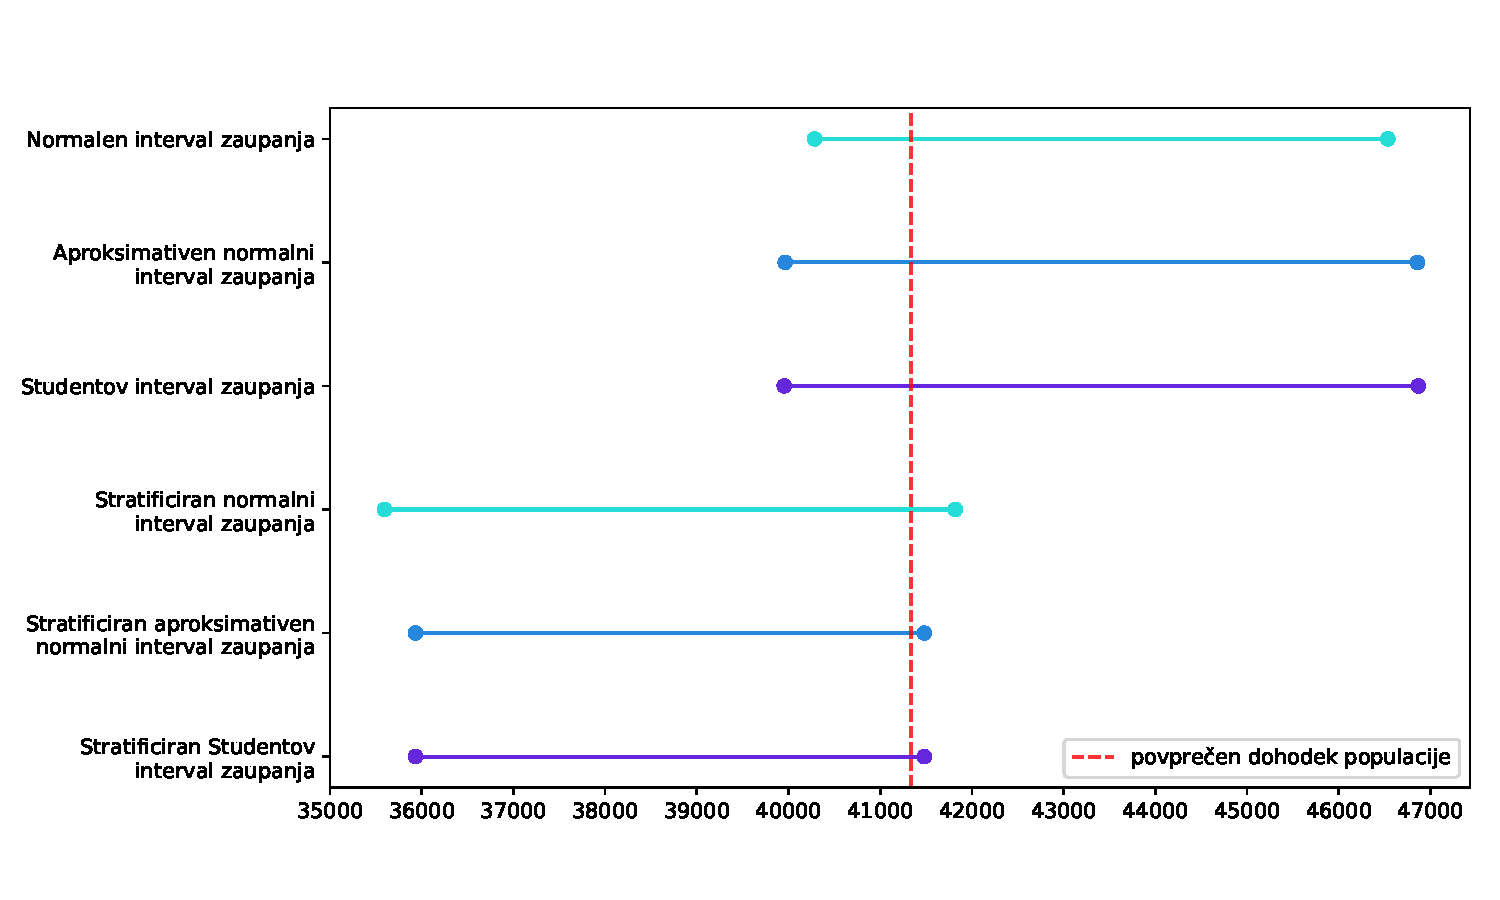
\includegraphics[width=\textwidth]{intervali_zaupanja.pdf}
    \caption{$95\%$ intervali zaupanja.}
\end{figure}

Zaključimo lahko, da je v tem primeru bolj ugodno stratificirati po četrtih, saj smo tako dobili ožje intevale zaupanja, kar nam bo omogočilo postaviti bolj natančne ocene povprečnega dohodka v Kibergradu. 

Do računskih razultatov pri tej nalogi smo prišli s pomočjo priloženih skript \texttt{naloga\_1a.ipynb} za točko a) in \texttt{naloga\_1b.ipynb} za točko b), ki analizirata isti enostaven slučajni vzorec $400$ enot (s proporcionalno alokacijo) iz datoteke \texttt{vzorec.csv}.

%-------------------------------------------------------------%
\section*{2. naloga}
%-------------------------------------------------------------%

Imamo vzorec $280$ palic, kjer smo vsaki od njih preizkusili lomljivost na petih mestih. Sumimo, da je število mest na katerih se je palica zlomila porazdeljeno $\bin(5,p)$, kar bo tudi naša osnovna ničelna domneva $H_0$.
\\

\noindent
\textbf{a)} Denimo, da osnovna ničelna domneva velja, po metodi največjega verjetja pa ocenimo parameter $p$. Vzemimo
\[
    L_1(p; x) = \mathsf{P}_p(X = x) = \binom{5}{x}p^x(1-p)^{5 - x},
\]
kjer je slučajna spremenljivka $X$ porazdeljena binomsko $\bin(5,p)$. \emph{Verjetje} bo tedaj funkcija
\[
    L(p; x_1, \ldots, x_n) = \prod_{i = 1}^n L_1(p; x) = \prod_{i = 1}^n \binom{5}{x_i}p^{x_i}(1-p)^{5 - x_i}.
\]
Cenilka za $p$ po metodi največjega verjetja bo torej tisti parameter, pri katerem je verjetje maksimalno. Ker je verjertje gladko odvisno od parametra $p \in (0,1)$ bomo ta ekstrem poiskali z odvodom, da bo računanje lažje, pa si bomo pomagali z logaritmom verjetja
\begin{multline*}
    \ell(p; x_1, \ldots, x_n) := 
    \log L(p; x_1, \ldots, x_n) \\ 
    = \sumin \log\binom{5}{x_i} + \sumin x_i\log(p) + \sumin(5 - x_i) \log(5 - p)
\end{multline*}
Z odvajanjem $\ell$ po $p$ dobimo
\[
    \ell'(p; x_1, \ldots, x_n) =
    \sumin \left( \frac{x_i}{p} - \frac{5 - x_i}{1 - p}\right) = 
    \sumin \frac{x_i - 5p}{p - p^2}.
\]
Ta odvod bo enak $0$ natanko tedaj, ko je $p = \frac{1}{5n} \sumin x_i$. Za vse $p \in (0,1)$ je $L(p; x_1, \ldots, x_n) > 0$, poleg tega pa velja
\[
    \lim_{p \downarrow  0} L(p; x_1, \ldots, x_n) = 0 \quad \text{ in } \quad 
    \lim_{p \uparrow  1} L(p; x_1, \ldots, x_n) = 0,
\]
za poljuben nabor $(x_1, \ldots, x_n) \in \{0,1,\ldots, 5\}^n$ razen, kadar so vsi $x_i$ enaki bodisi $0$ bodisi $5$, ko je maksimum verjetja $L$ dosežen na robu intervala $(0,1)$. To pomeni, da je $\frac{1}{5n} \sumin x_i$ res edini maksimum verjetja, torej lahko za cenilko $p$ vzamemo  
\[
    \hat{p} = \frac{\olsi{X}}{5}, \quad \text{ kjer je $\olsi{X}$ vzorčno povprečje.}  
\]

\noindent
\textbf{b)} S posplošenim Pearsonovim preizkusom hi kvadrat \cite[\S 9.5]{Rice} bomo v tem delu preizkusili ničelno domnevo, da ima število lomov porazdelitev $\bin(5,\hat{p})$, kjer je $\hat{p}$ cenilka za $p$ iz prejšnje točke. Opažanja poskusa so prikazana v tabeli. 
\begin{center}
\begin{tabular}{|| c | c ||}
    \hline
    št. lomov & št. palic \\
    \hline 
    \hline 
    0 & 157 \\
    \hline
    1 & 69 \\
    \hline
    2 & 35 \\
    \hline
    3 & 17 \\
    \hline
    4 & 1 \\
    \hline
    5 & 1 \\
    \hline
\end{tabular}
\end{center}

Ker Pearsonov preizkus zahteva, da je minimum po celicah najmanj 5, bomo zadnji dve celici pri $4$ in $5$ združili s celico $3$. Naj $O_i$ tako označuje število opažanj pri $i$-ti celici po zgornjem popravku (v tem primeru bo recimo $O_1 = 69$ in $O_3 = 19$). 

Za vsako od celic potrebujemo še pričakovane vrednosti, ki jih dobimo na podlagi porazdlitve pod ničelno hipotezo. V našem primeru označimo $p_i = \mathsf{P}(X = i)$ za $0 \leq i \leq 2$ ter $p_3 = \mathsf{P}(X = 3) + \mathsf{P}(X = 4) + \mathsf{P}(X = 5)$, kjer je $X \sim \bin(5, \hat{p})$ (da bo vsota vseh verjetnosti vselej $1$, smo kot posledico združitve celic $3$, $4$ in $5$ ustrezno prilagodili tudi verjetnost $p_3$). Pričakovana vrednost v vsaki od celic bo tedaj $E_i = n \cdot p_i$.

Testna statistika pri Pearsonovem preizkusu je 
\[
    \chi^2 = \sum_{i = 0}^3 \frac{(E_i - O_i)^2}{E_i}.
\]
Porazdeljena je s porazdelitvijo hi kvadrat z dvema prostostnima stopnjama, saj imamo $4$ celice in en parameter $\hat p$, ki smo ga ocenili na podlagi podatkov, torej $\chi^2 \sim \chi^2(2)$. Testna statistika izračunana na naših podatkih ima vrednost $\chi^2 = 44,149$, kar je večje od kvantila $F_{\chi^2(2)}\inv(1 - \alpha)$, tako pri stopnji tveganja $\alpha = 0,05$, kot tudi pri $\alpha = 0,01$, kjer je $F_{\chi^2(2)}$ kumulativna porazdelitvena funkcija porazdelitve $\chi^2(2)$. To pomeni, da našo ničelno hipotezo, ki pravi, da so lomi palic porazdeljeni binomsko $\bin(5, \hat{p})$, lahko na podlagi tega testa zavržemo.
\\

\noindent
\textbf{c)} Denimo, da imamo podanih $n$ neodvisnih opažanj $X_i \sim \bin(m_i, p_i)$ z znanimi parametri $m_i$ in neznanimi $p_i$. Ogledali si bomo kako s pomočjo razmerja verjetji preizkusimo ničelno domnevo, da so vsi parametri $p_i$ enaki proti alternativni domnevi, da temu ni tako. 

Naj bo \emph{funkcija verjetja} ali samo \emph{verjetje}
\[
    L(p_1, \ldots, p_n; x_1, \ldots, x_n)  = \prod_{i = 1}^n \binom{m_i}{x_i}p_i^{x_i} (1 - p_i)^{m_i - x_i}. 
\]
Naj bosta $\Theta = (0,1)^n$ in $\Theta_0 = \{(p_1, \ldots, p_n) \in \Theta \mid p_1 = \dots = p_n\}$. Zanima nas razmerje verjertji
\[
    \Lambda = \frac{\sup_{\bm{p} \in \Theta_0} L(\bm{p}; \bm{x})}{\sup_{\bm{p} \in \Theta} L(\bm{p}; \bm{x})},   
\]
za poljuben $\bm{x} \in \prod_{i = 1}^n\{0,1,\ldots, m_i\}$, kjer imamo krajše zapisano $\bm{p} =$ \linebreak $(p_1, \ldots, p_n)$ in $\bm{x} = (x_1, \ldots, x_n)$. Označimo še 
\begin{multline*}
    \ell(\bm{p}; \bm{x}) := 
    \log L(\bm{p}; \bm{x}) \\ = 
    \sumin \log \binom{m_i}{x_i} + \sumin x_i \log(p_i) + \sumin (m_i - x_i) \log(m_i - p_i)
\end{multline*}
logaritem verjetja.

Lotimo se najprej računanja imenovalca razmerja verjetji $\sup_{\bm{p} \in \Theta} L(\bm{p}; \bm{x})$. Ker je verjetje gladko odvisna funkcija parametra $\bm{p} \in \Theta \subseteq \R^n$, bo maksimum zavzela v stacionarni točki, kar pomeni, da bomo iskali ničle vseh pracialnih odvodov logaritma verjetja $\ell$, saj bo tako računanje lažje. Vidimo, da velja
\[
    \pdv{\ell}{p_j} (\bm{p}; \bm{x}) = 
    \frac{x_j}{p_j} - \frac{m_i - x_i}{m_i - p_i} = 
    \frac{x_i - m_i p_i}{p_i(1 - p_i)} = 0
\] 
natanko tedaj, ko je $p_i = \frac{x_i}{m_i}$. S podobnim argumentiranjem kot pri točki a) lahko zaključimo, da $\ell(\bm{p}; \bm{x})$ oziroma ekvivalentno $L(\bm{p}; \bm{x})$ doseže maksimum v točki $\bm{p} = (\frac{x_1}{m_1}, \dots, \frac{x_n}{m_n}) \in \ols\Theta$, ki pa je lahko tudi na robu domene $\Theta$. Če razumemo izraz $0^0$ kot $\lim_{x \downarrow 0}x^x = 1$, nam robne točke ne bodo povzročale težav. Tedaj je torej 
\[
    \sup_{\bm{p} \in \Theta} L(\bm{p}; \bm{x}) = 
    \prod_{i = 1}^n \binom{m_i}{x_i} \left(\frac{x_i}{m_i}\right)^{x_i} \left(\frac{m_i - x_i}{m_i}\right)^{m_i - x_i}.
\]

Sedaj se posvetimo še računanju števca $\sup_{\bm{p} \in \Theta_0} L(\bm{p}; \bm{x})$. Ožjo množico $\Theta_0$ lahko parametriziramo z $p \mapsto (p,\dots, p)$ za $p \in (0,1)$, torej bo $\ell(p, \dots, p; \bm{x})$ gladka funkcija zgolj enega parametra $p \in (0,1)$. Z odvajanjem po tem parametru dobimo 
\begin{multline*}
    \derivative{\ell}{p} (p, \dots, p; \bm{x}) = 
    \sumin \left(\frac{x_i}{p} - \frac{m_i - x_i}{1 - p}\right) \\ = 
    \sumin \frac{x_i - m_i p}{p(1-p)} = 
    \frac{\sumin x_i - p \sumin m_i}{p(1-p)},
\end{multline*}
kar ima ničlo natanko pri $p = \sumin x_i / \sumin m_i$. Prepričamo se lahko, da je v tej točki tudi zares maksimum $\ell$ na $\Theta_0$, torej imamo
\[
    \sup_{\bm{p} \in \Theta_0} L(\bm{p}; \bm{x}) = 
    \prod_{j = 1}^n \binom{m_j}{x_j} \left(\frac{\sumin x_i}{\sumin m_i}\right)^{x_j} \left(\frac{\sumin(m_i - x_i)}{\sumin m_i}\right)^{m_j - x_j}.
\]

Nazadnje je razmerje verjetji
\begin{align*}
    \Lambda &= 
    \frac{\sup_{\bm{p} \in \Theta_0} L(\bm{p}; \bm{x})}{\sup_{\bm{p} \in \Theta} L(\bm{p}; \bm{x})}  \\ 
    &= \prod_{j = 1}^n
    \frac{\binom{m_j}{x_j} \left(\frac{\sumin x_i}{\sumin m_i}\right)^{x_j} \left(\frac{\sumin(m_i - x_i)}{\sumin m_i}\right)^{m_j - x_j}}{\binom{m_j}{x_j} \left(\frac{x_j}{m_j}\right)^{x_j} \left(\frac{m_j - x_j}{m_j}\right)^{m_j - x_j}} \\ &= 
    \prod_{j = 1}^n
    \left(\frac{m_j}{x_j} \frac{\sumin x_i}{\sumin m_i}\right)^{x_j}
    \left(\frac{m_j}{m_j - x_j}\frac{\sumin(m_i - x_i)}{\sumin m_i}\right)^{m_j - x_j}.
\end{align*}
Porazdelitev te testne statistike je povsem neočitna in izkaže se, da si ne moremo niti pomagati z Wilksovim izrekom. saj za nekatere vzorce $\bm{x}$ funkcija $\bm{p}\mapsto L(\bm{p}; \bm{x})$ ni injektivna kot zahteva \cite[Theorem 1]{Ginestet}.

Zaradi tega izberemo drugačno pot. Simuliramo veliko vzorcev, recimo $N = 10.000$, iz porazdelitve pod ničelno hipotezo, na njih izvrednotimo testno statistiko, in potem na podlagi tega definiramo porazdelitev s pomočjo histograma. Realno os razdelimo na intervale širine 
\[
    \delta = \hat{\sigma} \sqrt[3]{\frac{24\sqrt{\pi}}{N}} \quad \text{ po Scottovem pravilu},
\]  
nato pa preštejemo koliko simuliranih testnih statistik pade v dani interval ($\hat{\sigma}$ predstavlja empirični standardni odklon).  Frekvenca -- tj. število simuliranih testnih statistik v danem intevalu deljeno z $N$ -- bo verjetnost, da slučajna spremenljivka zavzame vrednost ravno v tem intervalu. Natančneje to pomeni, da definiramo
\[
    \prob(\Lambda \in [\delta k, \delta(k+1))) := \frac{\text{\# simuliranih podatkov, ki pade v $[\delta k, \delta(k+1))$}}{N}
\]
za poljuben $k \in \Z$. Na podlagi tako definirane porazdelitve slučajne spremenljivke $\Lambda$, lahko izračunamo $p$-vrednost\footnote{$p$-vrednost opažanja je najmanjša možna meja pri kateri ničelno hipotezo zavrnemo z vsaj tolikšnjo stopnjo tveganja.} našega vzorca kot
\[
    p = \prob(\left\lvert \Lambda \right\rvert \geq \lambda_{stat}) = \prob(\Lambda \leq \lambda_{stat}) + \prob(\Lambda \geq \lambda_{stat})
\]
in ničelno domnevo pri stopnji tveganja $\alpha$ zavrnemo, če je $p < \alpha$.
\newline

\noindent
\textbf{d) } V zadnji točki te naloge uporabimo metodo \emph{bootstrap} kjer simuliramo $10.000$ vrednosti testne statistike $\Lambda$ pod ničelno domnevo, da naš vzorec sestavlja $280$ binomsko $\bin(5, \hat{p})$ porazdeljenih neodvisnih opažanj $X_i \sim \bin(5, \hat{p})$. Ob tem je $\hat{p} = \olsi{X}/5$ cenilka za $p$ po metodi največjega verjetja iz točke a). Glede na takšen vzorec se naša testna statistika poenostavi v 
\[
    \Lambda = \prod_{i = 1}^n \left(\frac{\olsi{X}}{X_i}\right)^{X_i} \left( \frac{5 - \olsi{X}}{5 - X_i}\right)^{5 - X_i},
\]
kjer je $\olsi{X} = \sumin X_i/n$ vzorčno povprečje. Na našem vzorcu testna statistika zavzame vrednost $\lambda_{stat} = 3,02 \cdot 10^{-97}$.

Test pokaže, da so prav vse vrednosti testne statistike na $10.000$ simuliranih vzorcih vedno večje od statistike $\lambda_{stat}$ izračunane na naših konkretnih podatkih, torej bomo ničelno hipotezo, da imajo vse palice zlome porazdeljene binomsko z enakimi parametri, s $p$-vrednostjo $0$ zavrgli.

Skripto, ki spada k tej nalogi, najdemo v datoteki \texttt{naloga\_2.ipynb}.

%-------------------------------------------------------------%
\section*{3. naloga}
%-------------------------------------------------------------%

V tej nalogi se bomo ukvarjali z analizo pulza pri študentih. V raziskavi so nekateri od študentov bili deležni fizične obremenitve (tek na mestu), pulz pa so jim izmerili pred in po obremeniti. Tudi študentom, ki niso tekli so za kontrolo dvakrat izmerili pulz. V naslednjih treh točkah bomo obravnavali kakšni dejavniki bi lahko vplivali na spremembo pulza med obema meritvama.
\\

\noindent
\textbf{a)} Za začetek bomo testirali ali je fizična obremenitev vplivala na spremembo pulza. Za spremembo pulza bomo vzeli razliko med zadnje izmerjenim pulzom in prvotno izmerjenim pulzom. Naj $\olsi{X}_1$ označuje povprečno spremembo pulza v skupini študentov deležnih obremenitve, $\olsi{X}_2$ pa povprečno spremembo pulza preostalih študentov. 

Za ničelno hipotezo si bomo zadali, da fizična obremenitev \emph{ne} vpliva na spremembo pulza. Pod to predpostavko bi bilo smiselno sklepati, da sta povprečji spremembe pulza v dveh skupinah študentov (z oziroma brez obremenitve) v splošnem enaki. Bolj formalno bomo torej testirali ničelno hipotezo
\[
    H_0 : \mu_1 = \mu_2,
\]
kjer $\mu_1$ predstavlja povprečno spremembo pulza splošnega študenta, ki je med meritvama opravljal fizično obremenitev, $\mu_2$ pa predstavlja spremembo pulza splošnega študenta, ki fiziče obremenitve ni izvajal (teh dveh podatkov ne poznamo). Z drugimi besedami bomo preizkušali ali nam medsebojno odstopanje vzorčnih povprečji $\olsi{X}_1$ in $\olsi{X}_2$ pojasni posebna izbira našega vzorca ali pa je za tem razlog, da obremenitev res vpliva na spremembo pulza. 

Predpostavljamo, da je pulz pri študentih porazdeljen normalno (kot je značilno za številne druge človeške karakteristike), torej bo tudi sprememba pulza kot razlika dveh normalnih podatkov normalno porazdeljena. Ob tem pa smo se odločili, da hipotezo preizkušamo z \emph{Welchevim $t$-testom} -- katerega opis še sledi, namesto s Studentovim $t$-testom. 
Razlog za tem pojasni veliko odstopanje varianc po skupinah. Če namreč označimo
\[
    s_1^2 = \frac{1}{n_1 - 1}\sum_{i = 1}^{n_1} (X_{1i} - \bar{X_1})^2
\]
nepristransko cenilko variance povprečne spremembe pulza v skupini študentov z obremenitvijo in podobno definiramo $s_2^2$ -- nepristransko cenilko variance povprečne spremembe pulza v skupini študentov, ki niso izvajali obremenitve, potem vidimo, da je na naših podatkih $s_1 > 2s_2$. Pri tem je $n_1 = 46$ študentov bilo deležnih fizične obremenitve, $n_2 = 63$ pa je bilo študentov brez obremenitve. 

Pri Welchevem $t$-testu je testna statistika podana kot
\[
    T = \frac{\olsi{X}_1 - \olsi{X}_2}{\sqrt{s_{\olsi{X}_1}^2 + s_{\olsi{X}_2}^2}},
    \quad \text{ kjer je }\quad s^2_{\olsi{X}_i} = \frac{s^2_i}{n_i}.
\]
Ta statistika je aproksimirana s Studentovo $t$-porazdelitvijo s približno 
\[
\hat{v} = \frac{\left(\frac{s_1^2}{n_1} + \frac{s_2^2}{n_2}\right)^2}{\frac{s_1^4}{n_1^2(n_1 - 1)} + \frac{s_2^4}{n_2^2(n_2 - 1)}} 
\]
prostostnimi stopnjami. To je Welch-Satterthwaitova enačba. Podobna je parametru, ki ga uporabljamo pri ocenjevanju vzorčnega povprečja pri stratificiranem vzorčenju, kjer ne poznamo stratumskih varianc (če sta stratuma samo dva). Podrobnosti o Welchevem $t$-testu najdemo v \cite{Welch} ali \cite[\S11]{Rice}.

Ker zdaj (vsaj približno) poznamo porazdelitev testne statistike, jo lahko izvrednotimo na naših podatkih in tako izračunamo $p$-vrednost našega opažanja, ki nam pove kako ekstremno je. Naš test bo obojestranski, torej izračunamo $p$-vrednost kot
\begin{multline*}
    p = \prob(\lvert T \rvert \geq t_{stat}) = 
    \prob(T \leq -t_{stat}) + \prob(T \geq t_{stat}) \\ = 
    2(1 - \prob(T < t_{stat})) = 
    2(1 - F_{\text{Student}(\hat{v})}(t_{stat})), 
\end{multline*}
kjer je $t_{stat}$ vrednost statistične spremenljivke na naših podatkih, $T \sim \text{Student}(\hat{v})$, $F_{\text{Student}(\hat{v})}$ pa je kumulativna porazdelitvena funkcija Studentove porazdelitve z $\hat v$ prostostnimi stopnjami. V tretjem enačaju smo upoštevali simetričnost Studentove porazdelitve okoli izhodišča $0$. Tako izračunana $p$-vrednost naših opažanj dosega velikostne rede $10^{-21}$, kar je \emph{zelo} malo in nam jasno omogoča zavreči ničelno hipotezo (pri stopnji tveganja $\alpha = 0,01$) ter sprejeti (dosti bolj smiselno) alternativno domnevo, da obremenitev vpliva na spremembo pulza študentov. 
\newline

\noindent
\textbf{b)} Empirično bi lahko  iz grafikona \ref{Sprememba pulza v odvisnosti od prvo izmerjenega pulza} sklepali, da študentje izbrani za obrmeneitev niso goljufali s tem, da niso tekli. Vsi, ki so imeli majhno spremembo pulza (recimo manj kot $20$) bodisi vadijo veliko in imajo natrenirano srce, ali pa so že prvo meritev opravili z neobičajno visokim pulzom in se jim zaradi tega ni mogel med obremenitvijo drastično dvigniti. Mogoče so hiteli na testiranje, ker so zamujali, in so zaradi tega že imeli povišan pulz ob prvem merjenju.

\begin{figure}[h]
    \begin{center}
        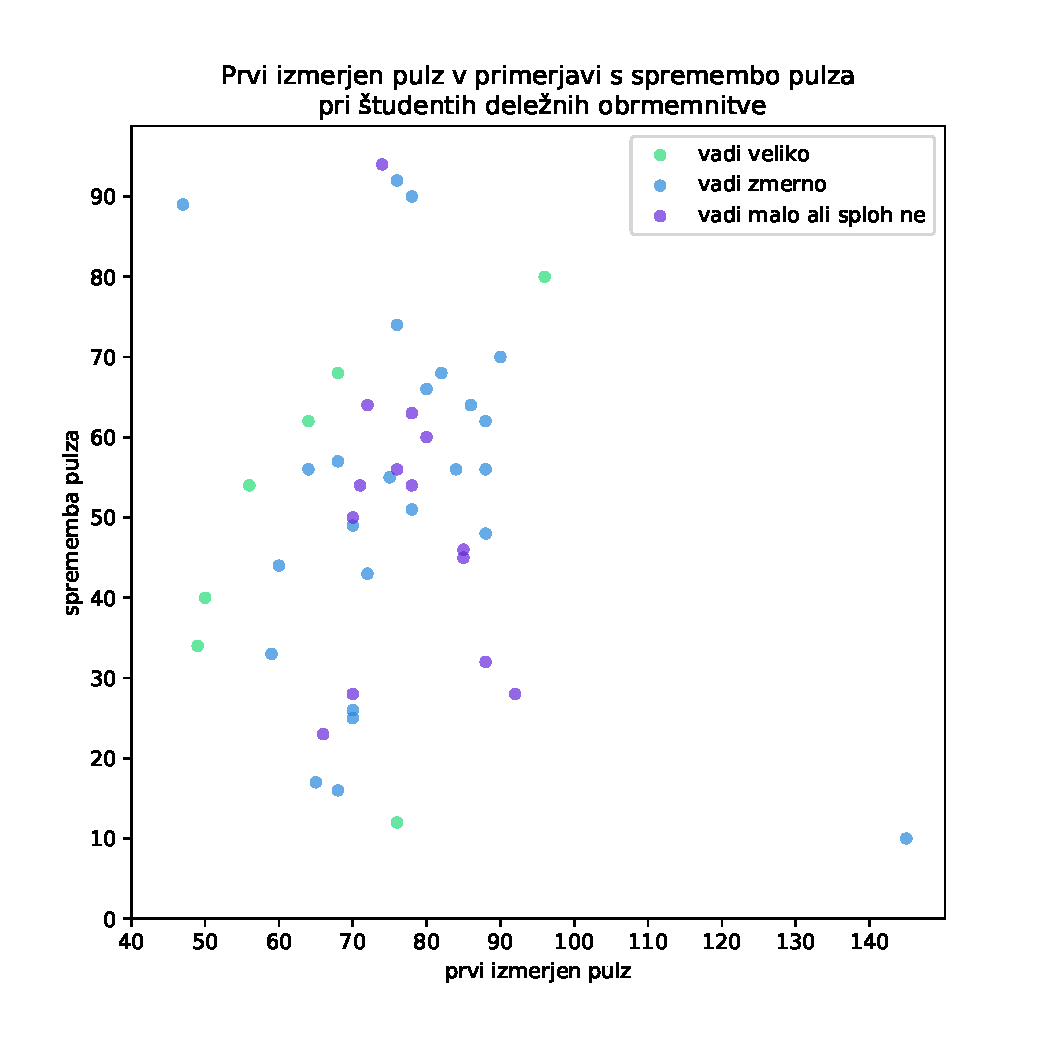
\includegraphics[scale=0.65]{pulz_vadba.pdf}
        \caption{
            Sprememba pulza v odvisnosti od prvo izmerjenega pulza.
            }
        \label{Sprememba pulza v odvisnosti od prvo izmerjenega pulza}
    \end{center}
\end{figure}

\noindent
\textbf{c)} Najprej testirajmo, če so vzorčne variance vseh treh skupin ne razlikujejo signifikantno (testiramo homogenost variance). V tem primeru, bomo uporabili analizo variance -- krajše ANOVA -- za preizkušanje ničelne domneve, da so vsa povprečja enaka, proti alternativni domnevi, da vsaj eno povprečje signifikantno odstopa od ostalih.
\newline

Homogenost variance bomo testirali z Levenovim testom, ki je v resnici zgolj modifikacija testa ANOVA, zato si najprej poglejmo kako deluje ta. Glavni cilj analize variance je ugotoviti ali se povprečja po skupinah med sabo signifikantno razlikujejo ali ne. Recimo, da imamo danih $n$ vzorecev $Y_{ij}$, za $1 \leq j \leq n_i$, $1 \leq i \leq k$ razdeljenih na $k$ skupin, kjer vsaka skupina vsebuje $n_i$ vzorcev. Z $\ols{Y}_{i\cdot}$ označimo povprečje znotraj $i$-te skupine, $\ols{Y}$ pa naj bo vzorčno povprečje vseh podatkov. Osnovna ideja tega testa bo pogledati razmerje variabilnosti vzorca med skupinami in variabilnosti vzorca v skupinah samih. Natančneje definirajmo 
\[
    \sigma^2_B = \sum_{i = 1}^k \frac{n_i (\ols{Y}_{i \cdot} - \ols{Y})^2}{k-1},
\]
imenovano tudi \emph{pojasnjena varianca} -- varianca med skupinami vzorca, ter
\[
    \sigma^2_W = \sum_{i = 1}^k \sum_{j = 1}^{n_i} \frac{(Y_{ij} - \ols{Y}_{i \cdot})^2}{n - k},
\] 
ki se imenuje \emph{nepojasnjena varianca} -- varianca znotraj skupin vzorca. Testno statistiko tako vpeljemo kot
\[
    F = \frac{\sigma^2_B}{\sigma^2_W}.
\]  
Izkaže se, da sta pojasnjena in nepojasnjena varianca hi kvadrat porazdeljeni in sicer je $(k-1)\sigma^2_B \sim \chi^2(k - 1)$ ter $(n-k)\sigma^2_W \sim \chi^2(n - k)$. Tako spoznamo novo porazdelitev imenovano \emph{$F$-porazdelitev s parametroma $d_1$ in $d_2$}, ki je definirana kot porazdelitev slučajne spremenljivke
\[
    \frac{U_1/d_1}{U_2/d_2} \sim F(d_1, d_2),
\] 
kjer sta $U_1 \sim \chi^2(d_1)$ in $U_2 \sim \chi^2(d_2)$ neodvisni. Ničelno hipotezo tedaj zavrnemo, če je $p$-vrednost, ki jo izračunamo kot
\[
    p = \prob(F \geq f_{stat}) = 1 - F_{F(k-1, n - k)}(f_{stat})
\]
kjer je $F \sim F(k - 1, n - k)$, $F_{F(k-1, n - k)}$ kumulativna porazdelitvena funkcija te spremenljivke, $f_{stat}$ pa vrednost statistične spremenljivke izračunane na našem vzorcu, manjša od zadane stopnje tveganja $\alpha$.


Omenili smo že, da je Levenov test zgolj prilagojena različica tega testa in sicer spremenljivke $\ols{Y}_{ij}$ zamenjamo z $Z_{ij} = \lvert Y_{ij} - \ols{Y}_{i \cdot}\rvert$. Tako dobimo testno statistiko 
\[
    W = \frac{n - k}{k - 1} \cdot \frac{\sum_{i = 1}^k n_i (\olsi{Z}_{i \cdot} - \olsi{Z})^2}{\sum_{i = 1}^k \sum_{j = 1}^{n_i} (Z_{ij} - \ols{Z}_{i \cdot})^2},
\] 
ki je $F(k - 1, n - k)$-porazdeljena. V enačbi $\olsi{Z}_{i \cdot}$ predstavlja povprečje spremenljivk $Z_{ij}$ v $i$-ti skupini, $\olsi{Z}$ pa je povprečje vseh $Z_{ij}$.
\newline

S $p$-vrednostjo $0,660$, lahko po Levenovem testu sklepamo, da imajo tri skupine študentov z obremenitvijo glede na to koliko vadijo nesignifikantno različne variance spremembe pulza. Z drugimi besedami je sprememba pulza v vseh treh skupinah približno enako razpršena okrog povprečja, kot lahko empirično do neke mere potrdimo iz grafikona \ref{Razprsenost spremembe pulza po skupinah glede na vadbo}.

\begin{figure}[h]
    \begin{center}
        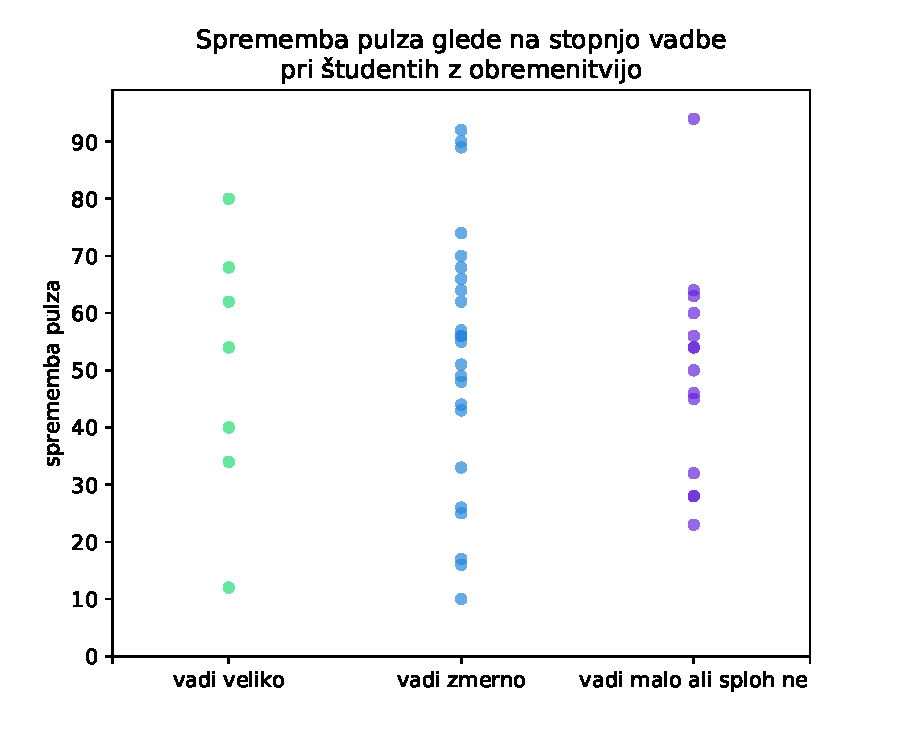
\includegraphics[scale=0.7]{varianca_vadba.pdf}
        \caption{
            Razpršenost spremembe pulza po skupinah glede na vadbo.
            }
        \label{Razprsenost spremembe pulza po skupinah glede na vadbo}
    \end{center}
\end{figure}


Sedaj bomo za študente, ki so bili deležni obrmemenitve, testirali ničelno hipotezo
\[
H_0: \text{vadba nima vpliva na spremembo pulza}.
\]
Z drugimi besedami, bi bilo smiselno za ničelno hipotezo vzeti $H_0 : \mu_1 = \mu_2 = \mu_3$, kjer so $\mu_1, \mu_2, \mu_3$ povprečja splošnih študentov, ki vadijo veliko, zmerno oziroma malo ali skoraj nič. To hipotezo bomo testirali z analizo variance. Ta test prepostavlja naslednje:
\begin{itemize}
    \item Ekspirimentalna napaka pri merjenju podatkov je približno normalno porazdeljena (to bomo privzeli).
    \item Homogenost variance (to nam je potrdil Levenov test zgoraj).
    \item Posamezne enote vzorca so neodvisne drug od druge (tudi to bomo privzeli).
\end{itemize}

Vidimo, da je $p$-vrednost $0,907$ precej velika, kar pomeni, da bi vsaj tako ekstremen rezulat, kot je naš, dobili dokaj pogosto -- naš vzorec torej ni preveč ekstremen. Na podlagi tega testa lahko tako statistično sklepamo, da je ničelna hipoteza resnična, kar pomeni, da vadba nima vpliva na spremembo pulza pri študentih z obrmenitvijo.

Skripto za izračune in analizo zadnje naloge najdemo v datoteki \linebreak \texttt{naloga\_3.ipynb}.

\begin{thebibliography}{99}

    \bibitem{Rice}
    J.~Rice, \emph{Mathematical statistics \& data analysis}, third edition, Duxbury, 2007.

    \bibitem{Ginestet}
    C.~E.~Ginestet, \emph{MA 782 Hypothesis Testing: Consistency and Normality of MLE}, [ogled 21.~8.~2021], dostopno na \url{http://math.bu.edu/people/cgineste/classes/ma782/p/w1_1.pdf}.

    \bibitem{Welch}
    \emph{Welch's $t$-test}, v: Wikipedia, The Free Encyclopedia, [ogled 21.~8.~2021], dostopno na \url{https://en.wikipedia.org/wiki/Welch%27s_t-test}.
    
\end{thebibliography}

\end{document}